

\documentclass[aspectratio=169]{beamer}
\usetheme{CambridgeUS}

\setbeamertemplate{navigation symbols}{}%remove navigation symbols
\setbeamersize{text margin left=30pt, text margin right=30pt}

\usepackage{amsmath}
\usepackage{amsfonts}
\usepackage{algorithm}
\usepackage[noend]{algpseudocode} 
\usepackage{tikz}
\usetikzlibrary{arrows}

\newcommand{\emm}{\mathcal{M}}
\newcommand{\dbd}{\mathbb{N}^{|\chi|}}

\title{Introduction to Differential Privacy}
\author{J.T. Cho}
\institute{CIS700-003 | University of Pennsylvania}
\date{March 2017}

\begin{document}

\begin{frame}
\titlepage
\end{frame}

\begin{frame}
\frametitle{Introduction}

Data collection in the modern era.\\~\\

Want to be able to compute statistics and respond to queries on sensitive datasets.\\~\\

\emph{Paradox.} Can we learn information about a population without learning anything about the individual?
\end{frame}

\begin{frame}
\frametitle{Privacy Accuracy Tradeoff}
\begin{center}
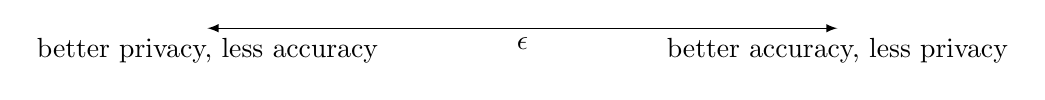
\begin{tikzpicture}
\draw[latex-latex] (-4,0) -- (4, 0);
\draw[shift={(-4, 0)}, color=black] (0pt,0pt) -- (0pt, 0pt) node[below] {better privacy, less accuracy};
\draw[shift={(0, 0)}, color=black] (0pt,0pt) -- (0pt, 0pt) node[below] {$\epsilon$};
\draw[shift={(4, 0)}, color=black] (0pt,0pt) -- (0pt, 0pt) node[below] {better accuracy, less privacy};
\end{tikzpicture}
\end{center}
\end{frame}

\begin{frame}
\frametitle{Privacy Preserving Data Analysis}

\begin{itemize}
  \item Data can not remain fully anonymized and remain useful. (e.g. linkage attack)
  \item Re-identification of anonymized records is not the only risk. (even without direct linkage, incriminating information can still be found)
  \item Can we query audit?
  \item Summary statistics are not safe, either.
  \item Ordinary traits can still be used to indirectly reveal sensitive properties.
\end{itemize}
\end{frame}

\begin{frame}
\frametitle{Differencing Attack}

\emph{Example.} You are given a medical database of individuals and the knowledge that a person $X$ is in the database. If you aren't allowed to query for $X$'s properties directly, how would you determine whether $X$ has diabetes?
\end{frame}

\begin{frame}
\frametitle{Intuitively Formalizing Privacy}

\textbf{Desiderata.} An individual's risk is not increased significantly by opting into a study.\\~\\

In other words, individuals should have \textit{plausible deniability}.\\~\\
%% Suppose we want to test for the percentage of smokers in a population
%% of people.
\end{frame}

\begin{frame}
\frametitle{A Game of Plausible Deniability}
  Suppose we want to test for the percentage of smokers in a population of people.\\~\\

  \textbf{Goal.} Design a protocol for surveying people so they may claim plausible deniability of being a smoker.
\end{frame}

%% Randomized Response
\begin{frame}
\frametitle{Randomized Response}
\textbf{Protocol.}\\~\\
\begin{enumerate}
  \item Flip fair coin.
  \item If tails, respond truthfully.
  \item If heads, flip second coin, respond \texttt{Yes} if heads, \texttt{No} if tails.
\end{enumerate}

How does this give us plausible deniability?
\end{frame}

%% Randomized Response, cont.
\begin{frame}
\frametitle{Randomized Response, cont.}
  Plausibility deniability of any outcome gives us privacy - can't single out an individual. \\~\\

  Adding uncertainty to query output in the form of randomness/noise allows us to achieve this.\\~\\

  The issue is then to analyze the noisy data to derive an accurate result!

  %% Do analysis of expectations here.
\end{frame}

%% Intuitively Defining Differential Privacy
\begin{frame}
\frametitle{Intuitively Defining Differential Privacy}

We are given a database, an individual, and a mechanism which processes queries.\\~\\

This mechanism should with high probability output the same result whether or not the individual's information is in the database!
\end{frame}

\begin{frame}
\frametitle{Model of Computation}

\textbf{Definition.} (Probability Simplex) Given a discrete set $B$, the probability simplex over $B$ denoted $\Delta(B)$ is

$$\Delta(B) = \bigg\{ x \in \mathbb{R}^{|B|}\;:\; x_i \geq 0\;\forall i, \sum_{i=1}^{|B|} x_i = 1\bigg\}$$

In plain English, $\Delta(B)$ is the set of all probability vectors of length $|B|$ that sum to $1$.
\end{frame}

%% Model of Computation, cont.
\begin{frame}
\frametitle{Model of Computation, cont.}

\textbf{Definition.} (Mechanism) A mechanism $\emm$ with domain $A$ and range $B$ is associated with the mapping $\emm\;:\;A \rightarrow \Delta(B)$. On input $a \in A$, the mechanism $\emm$ outputs $\emm(a) = b$ with probability $(\emm(a))_b$ for each $b \in B$.\\~\\

The probability is taken over the randomness of the mechanism (coin flips).\\~\\

Our goal is to find a differentially private mechanism!

\end{frame}

%% Model of Computation, cont.
\begin{frame}
\frametitle{Model of Computation, cont.}

A database will be represented as a `histogram' vector $x \in \dbd$, counting the frequency of each element from the universe $\chi$.\\~\\

\textbf{Definition.} (Distance Between Databases) The $\ell_1$ norm of a database $x$ is denoted $||x||_1$, defined as

$$||x||_1 = \sum_{i=1}^{|\chi|} |\chi_i|$$

The $\ell_1$ distance between $2$ databases $x, y$ is $||x-y||_1$, the number of records differing between $x$ and $y$.
\end{frame}

%% Differential Privacy
\begin{frame}
\frametitle{Differential Privacy}

\textbf{Definition.} A mechanism $\emm$ on a database with domain $\dbd$ is $(\epsilon, \delta)$-differentially private if $\forall S \subseteq \text{Range}(\emm)$ and $\forall x,y \in \dbd$ such that $||x-y||_1 \leq 1$,

$$\Pr(\emm(x) \in S) \leq \exp(\epsilon) \Pr(\emm(y) \in S) + \delta$$

with the probability space over the coin flips in the mechanism $\emm$.\\~\\

If $\delta = 0$, $\emm$ is $\epsilon$-differentially private.
\end{frame}

%% Differential Privacy, cont.
\begin{frame}
\frametitle{Understanding the Definition}

Consider the singleton set $\{s\} \subseteq \text{Range}(\emm)$ - $s$ is an example output of $\emm$.\\~\\

If $\emm$ is $\epsilon$-diff. private, the probability of outputting $s$ on $x$ is at most $e^{\epsilon}$ times the probability of outputting $s$ on any neighboring database $y$.\\~\\
\end{frame}

%% Understanding the Definition, cont.
\begin{frame}
\frametitle{Understanding the Definition, cont.}
In other words, the definition states that the probability of any output of $\emm$ is within an $e^{\epsilon}$ factor of whether or not an individual is included in the database.\\~\\

The smaller $\epsilon$ is, the stronger the `privacy' guarantee!
\end{frame}

%% Randomized Response, Revisited
\begin{frame}
\frametitle{Randomized Response, Revisited}
\textbf{Claim.} Randomized response is $(\ln 3, 0)-$differentially private.\\~\\

\textit{Proof.} Let the databases be drawn from universe $\{0, 1\}$ and the mechanism range $\text{Range}(\emm) = \{0, 1\}$.

$$\Pr(\text{Response = No} \mid \text{Truth = No}) = \Pr(M(0) \in \{0\}) = 3/4$$
$$\Pr(\text{Response = No} \mid \text{Truth = Yes}) = \Pr(M(1) \in \{0\}) = 1/4$$

If $\epsilon = \ln 3$, 
\begin{align*}
  \Pr(M(0) \in \{0\}) = 3/4 \leq \exp(\epsilon) \Pr(M(1) \in \{0\}) = 3/4\\
  \Pr(M(1) \in \{0\}) = 1/4 \leq \exp(\epsilon) \Pr(M(0) \in \{0\}) = 9/4\\
\end{align*}
\end{frame}

\begin{frame}
\frametitle{Benefits of Differential Privacy}
\begin{itemize}
  \item Protection against arbitrary risks, not just re-identification
  \item Neutralization of linkage attacks (past/present/future), and auxiliary information
  \item Quantification of privacy loss
  \item Composition (combining differentially private mechanisms)
  \item Group Privacy
  \item Closure under Post-Processing (differential privacy can't be reduced after)
\end{itemize}
\end{frame}

\begin{frame}
\frametitle{What Differential Privacy Does Not Promise}

\begin{itemize}
  \item Does not create privacy where there was none
  \item Does not guarantee that one's secrets will be protected. Aggregate conclusions can still reflect on the individual. (Merely occludes specifics of a person's participation)
\end{itemize}
\end{frame}


%%
\begin{frame}
\frametitle{Finding an $\epsilon$-private Mechanism}
Our intuition from before is that adding noise to original data gives `privacy'.\\~\\

Instead of coin flips, what if we chose a different probability distribution and added a dependence on $\epsilon$?\\~\\

We also want to be able to control how sensitive the mechanism is to changes in the database (i.e. should including a single individual result in a big change in the output?)
\end{frame}

%% Laplace Distribution
\begin{frame}
\frametitle{Laplace Distribution}

\textbf{Definition.} (Laplace Distribution) The Laplace distribution centered at 0 with scale $b$ has the pdf,

$$\text{Lap}(x\mid b) = \frac{1}{2b} \exp(-\frac{|x|}{b})$$

and variance,

$$\sigma^2 = 2b^2$$

Often written as Lap$(b)$ for short.
\end{frame}

%% l1 sensitivity
\begin{frame}
\frametitle{$\ell_1$ sensitivity}

We define \textbf{numeric queries} to be functions $f: \dbd \rightarrow \mathbb{R}^k$ (i.e. taking in a database and outputting a $k$-long real-valued vector).\\~\\

\textbf{Definition.} ($\ell_1$-sensitivity) The $\ell_1$-sensitivity of a numeric query $f$ is: 

$$\Delta f: \max_{\substack{x,y \in \dbd\\ ||x-y||_1 = 1}} ||f(x) - f(y)||_1$$

The $\ell_1$-sensitivity captures the magnitude by which an individual's data can change the function $f$ in the worst case.
\end{frame}

%% Laplace Mechanism
\begin{frame}
\frametitle{Laplace Mechanism}

\textbf{Definition.} (Laplace Mechanism) Given any function $f\;:\; \dbd \rightarrow \mathbb{R}^k$, the Laplace mechanism is defined,

$$\emm_L(x, f(\cdot), \epsilon) = f(x) + (Y_1, Y_2, \dots, Y_k)$$\\~\\

where the $Y_i$ are i.i.d. drawn from $\text{Lap}(\Delta f/\epsilon)$.
\end{frame}

%% Laplace Mechanism, cont.
\begin{frame}
\frametitle{Laplace Mechanism, cont.}

\textbf{Theorem.} The Laplace mechanism preserves $(\epsilon, 0)$-differential privacy.\\~\\

\emph{Sketch of Proof.} Consider any two databases $x$ and $y$ that differ in at most $1$ record and a database function $f$. \\~\\

Consider the probabilities of getting some arbitrary value $z$ from evaluating the mechanism $\emm_L(x, f, \epsilon)$ and $\emm_L(y, f, \epsilon)$.\\~\\

Taking the ratio and using the Laplace distribution pdf, use a series of inequality bounds to demonstrate that the ratio is bounded by $\exp(\epsilon)$.

%% To be shown on the chalkboard.
\end{frame}

%% Laplace Mechanism Example
\begin{frame}
\frametitle{Example}

\textbf{Input.} Database $x$ of medical information of $N$ records.\\~\\

\textbf{Goal.} Compute proportion of smokers in a differentially private way.\\~\\

$g(x) = [\#$ of smokers in $x]/N$.\\~\\

For any two databases differing in a single element, what is the largest amount that the proportion can change by?
\end{frame}

\begin{frame}
\frametitle{Exponential Mechanism}

Designed for non-numerical queries and cases where adding noise directly to the output is undesirable.\\~\\

Utility function $u\;:\; \dbd \times \mathcal{R} \rightarrow \mathbb{R}$, maps database/output pairs to utility scores.\\~\\

\emph{Sensitivity of $u$:}

$$\Delta u = \max_{r \in \mathcal{R}} \max_{x,y:||x-y||_1 \leq 1} |u(x,r) - u(y,r)|$$

\emph{Intuition.} Output element of $\mathcal{R}$ with maximum possible utility.\\~\\
\end{frame}

\begin{frame}
\frametitle{Exponential Mechanism, cont.}

\textbf{Definition.} (Exponential Mechanism) The exponential mechanism $\emm_E(x, u, \mathcal{R})$ selects and outputs an element $r \in \mathcal{R}$ with probability proportional to $\exp(\frac{\epsilon u(x,y)}{2\Delta u})$.
\end{frame}

\begin{frame}
\frametitle{Exponential Mechanism, cont.}

\textbf{Theorem.} The exponential mechanism preserves $(\epsilon, 0)$-differential privacy.
\end{frame}

\begin{frame}
\frametitle{Differentially Private Online Learning}

\textbf{Context.} You want to invest in the stock market and have assembled a panel of experts. Each day, you can pick one expert's choice of stock to invest in.\\~\\

\textbf{Goal.} Each day, pick experts such that after a period of time you do almost as well as the best expert!\\~\\
\end{frame}

\begin{frame}
\frametitle{Differentially Private Online Learning, cont.}

\textbf{Scenario.} Each day $t = 1, \dots, T$.
\begin{enumerate}[(a)]
  \item Choose expert $a_t \in \{1, \dots, k\}$.
  \item Observe loss $\ell_i^t \in [0,1]$ for each expert $i \in \{1, \dots, k\}$ and experiences loss $\ell_a^t$.\\~\\

  For sequence of losses $\ell^{\leq T} = \{\ell^k\}_{t=1}^T$,
  $$L_i(\ell^{\leq T}) = \frac{1}{T} \sum_{t=1}^T \ell_i^t \text{    (total avg. loss of expert $i$)}$$
  $$L_A(\ell^{\leq T}) = \frac{1}{T} \sum_{t=1}^T \ell_{a_t}^t \text{    (total avg. loss of algorithm)}$$
\end{enumerate}
\end{frame}

\begin{frame}
\frametitle{No Regret Learning}

$$\text{Regret}(A, \ell^{\leq T}) = L_A(\ell^{\leq T}) - \min_i L_i (\ell^{\leq T})$$\\~\\

Regret is the difference between the loss incurred by the algorithm and the loss of the best expert.\\~\\

\textbf{Goal.} Design algorithms guaranteeing that \emph{for all} possible loss sequences $\ell^{\leq T}$, even adversarilly chosen,

$$\text{Regret} \rightarrow 0 \text{ as } T\rightarrow \infty$$
\end{frame}

\begin{frame}
\frametitle{Random Weighted Majority Algorithm}

\textbf{Input.} Stream $\sigma_{\ell}$ of losses $\ell^1, \ell^2, \dots$\\~\\

\textbf{Output.} Stream of actions $a_1, a_2, \dots$\\~\\

\begin{algorithm}[H]
\begin{algorithmic}
  \Procedure{RWM}{$\eta$}
  \For{$i \in \{1, \dots, k\}$, let $w_i \gets 1$}
  \EndFor
  \For{$t=1,\dots,$}
    \State{Choose action $a_t = i$ with probability proportional to $w_i$.}
    \State{Observe $\ell^t$ and set $w_i \gets w_i \cdot \exp(-\eta \ell_i^t), \forall i \in [k]$}
  \EndFor
  \EndProcedure
\end{algorithmic}
\end{algorithm}
\end{frame}

\begin{frame}
\frametitle{Random Weighted Majority Algorithm, cont.}

\textbf{Theorem.} for any adversarially chosen sequence of losses of length $T$, $\ell^{\leq T} = (\ell^1, \dots, \ell^T)$, the R.W.M. algorithm with update parameter $\eta$ has guarantee:

$$E[\text{Regret}(\text{RWM}(\eta), \ell^{\leq T})] \leq \eta + \frac{\ln(k)}{nT}$$

Choosing $\eta = \sqrt{\ln k/T}$ yields

$$E[\text{Regret(RWM}(\eta), \ell^{\leq T})] \leq 2\sqrt{\frac{\ln k}{T}}$$

which tends to $0$ as $T$ goes to $\infty$.
\end{frame}

\begin{frame}
\frametitle{Differentially Private Online Learning, cont.}

Can we do the same process but in a differentially private way?\\~\\

What should our ``input database'' be? Our output?
\end{frame}

\begin{frame}
\frametitle{Differentially Private Online Learning, cont.}
\textbf{Input Database.} Collection of loss vectors $\ell^{\leq T} = (\ell^1, \dots, \ell^T)$. Neighboring databases $\ell^{\hat{\leq}T}$ differs in entire vector in $1$ timestep.\\~\\

\textbf{Output.} Sequence of actions chosen by the algorithm, $a_1,\dots, a_T$.
\end{frame}

\begin{frame}
\frametitle{Random Weighted Majority Algorithm, cont.}

We present the same algorithm from before, presented in a slightly different way.

\begin{algorithm}[H]
\begin{algorithmic}
  \Procedure{RWM}{$\eta$}
  \For{$t=1,\dots,$}
    \State{Choose action $a_t = i$ with probability proportional to $\exp(-\eta \sum_{j=1}^{t-1}\ell_i^j)$.}
    \State{Observe $\ell^t$.}
  \EndFor
  \EndProcedure
\end{algorithmic}
\end{algorithm}

This is the exponential mechanism with quality score $q(i, \ell^{< T}) \sum_{j=1}^{t-1} \ell_i^j$.
\end{frame}

\begin{frame}
\frametitle{Differential Privacy and RWM}

\textbf{Theorem.} For a sequence of losses of length $T$, the algorithm RWM($\eta$) with $\eta = \frac{\epsilon}{\sqrt{32 T \ln(1/\delta)}}$ is ($\epsilon, \delta)$-differentially private.
\end{frame}

\end{document}
